\begin{tcbitemize}[raster columns=4, raster equal height=rows,
        size=small,colback=colorrds!5!white,
        colframe=colorrds!35!white,colbacktitle=colorrds!50!white,
        fonttitle=\centering\bfseries,title={Criterio \# \thetcbrasternum}]
    \tcbitem
    \begin{center}\bfseries
        Lado-lado-lado\\
        (LLL)
    \end{center}
    Cuando los tres pares de lados correspondientes son congruentes, los triángulos son congruentes.

    \begin{figure}[H]
        \centering
        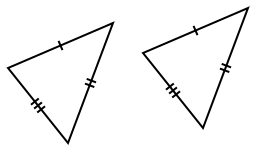
\includegraphics[width=0.9\textwidth]{../images/criterioLLL}
        \caption{}
        \label{fig:criterioLLL}
    \end{figure}

    \tcbitem
    \begin{center}\bfseries
        Lado-ángulo-lado\\ (LAL)
    \end{center}
    Cuando dos pares de lados correspondientes y los ángulos entre ellos son congruentes, los triángulos son congruentes.

    \begin{figure}[H]
        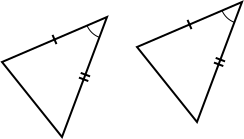
\includegraphics[width=0.9\textwidth]{../images/criterioLAL}
        \caption{}
        \label{fig:criterioLAL}
    \end{figure}

    \tcbitem
    \begin{center}\bfseries
        Ángulo-lado-ángulo\\ (ALA)
    \end{center}
    Cuando dos pares de ángulos correspondientes y los lados entre ellos son congruentes, los triángulos son congruentes.
    \begin{figure}[H]
        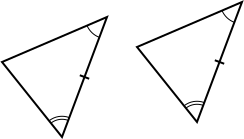
\includegraphics[width=0.9\textwidth]{../images/criterioALA}
        \caption{}
        \label{fig:criterioALA}
    \end{figure}

    \tcbitem[]  \begin{center}\bfseries
        Lado-lado-lado \\ (AAL)
    \end{center}
    Cuando dos pares de ángulos correspondientes y un par de lados correspondientes (no entre los ángulos) son congruentes, los triángulos son congruentes.

    \begin{figure}[H]
        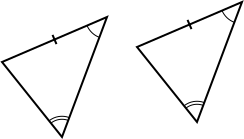
\includegraphics[width=0.9\textwidth]{../images/criterioAAL}
        \caption{}
        \label{fig:criterioAAL}
    \end{figure}
\end{tcbitemize}